\section{CHAPTER 6: GENERATOR \cite{j420}}
\begin{figure}[h!]
    \centering
    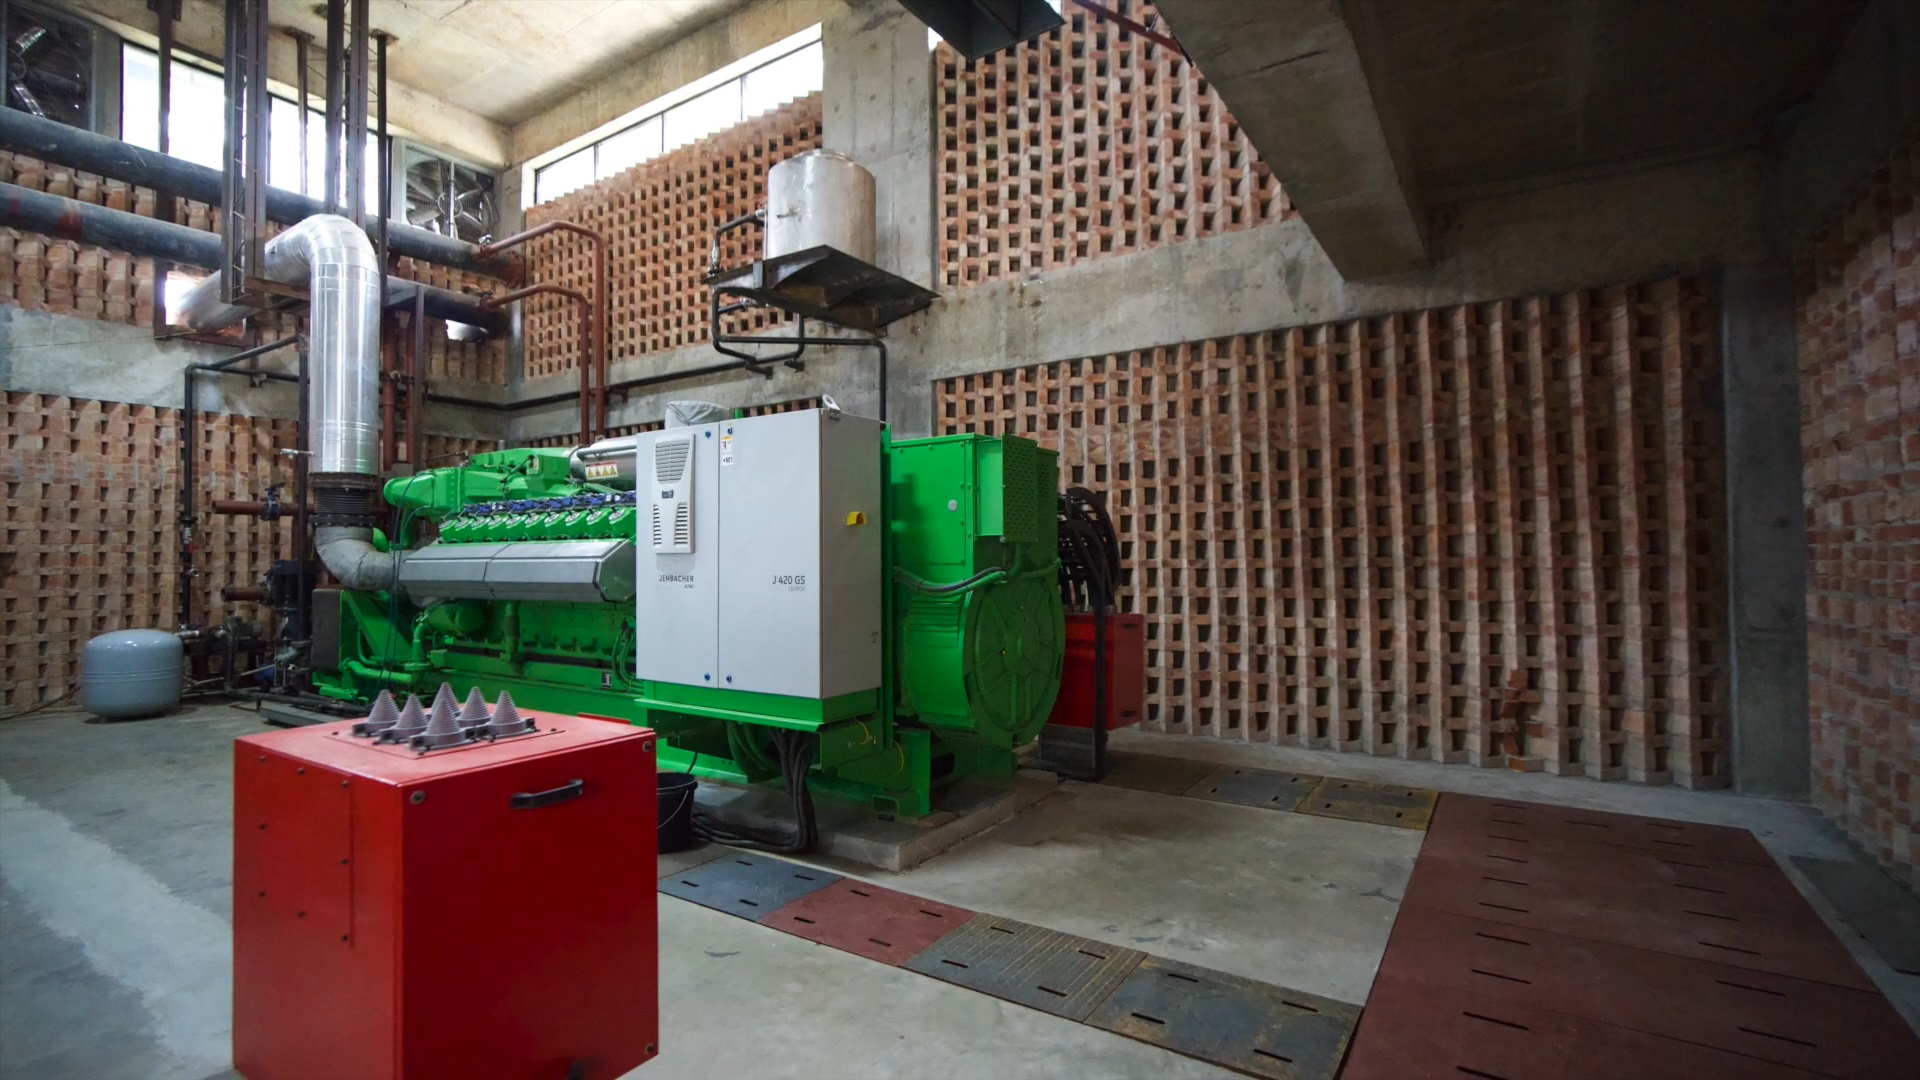
\includegraphics[width=1\linewidth]{figs/generator.jpg}
    \caption{Generator machine}
    \label{fig:generator}
\end{figure}

Generators play a crucial role in the textile industry by providing a reliable source of power. They ensure that the production process is not interrupted due to power outages, which can be costly and time-consuming. The generator machine shown in Figure \ref{fig:generator} is typically used in small to medium-sized textile companies to maintain continuous operations.

\begin{figure}
    \centering
    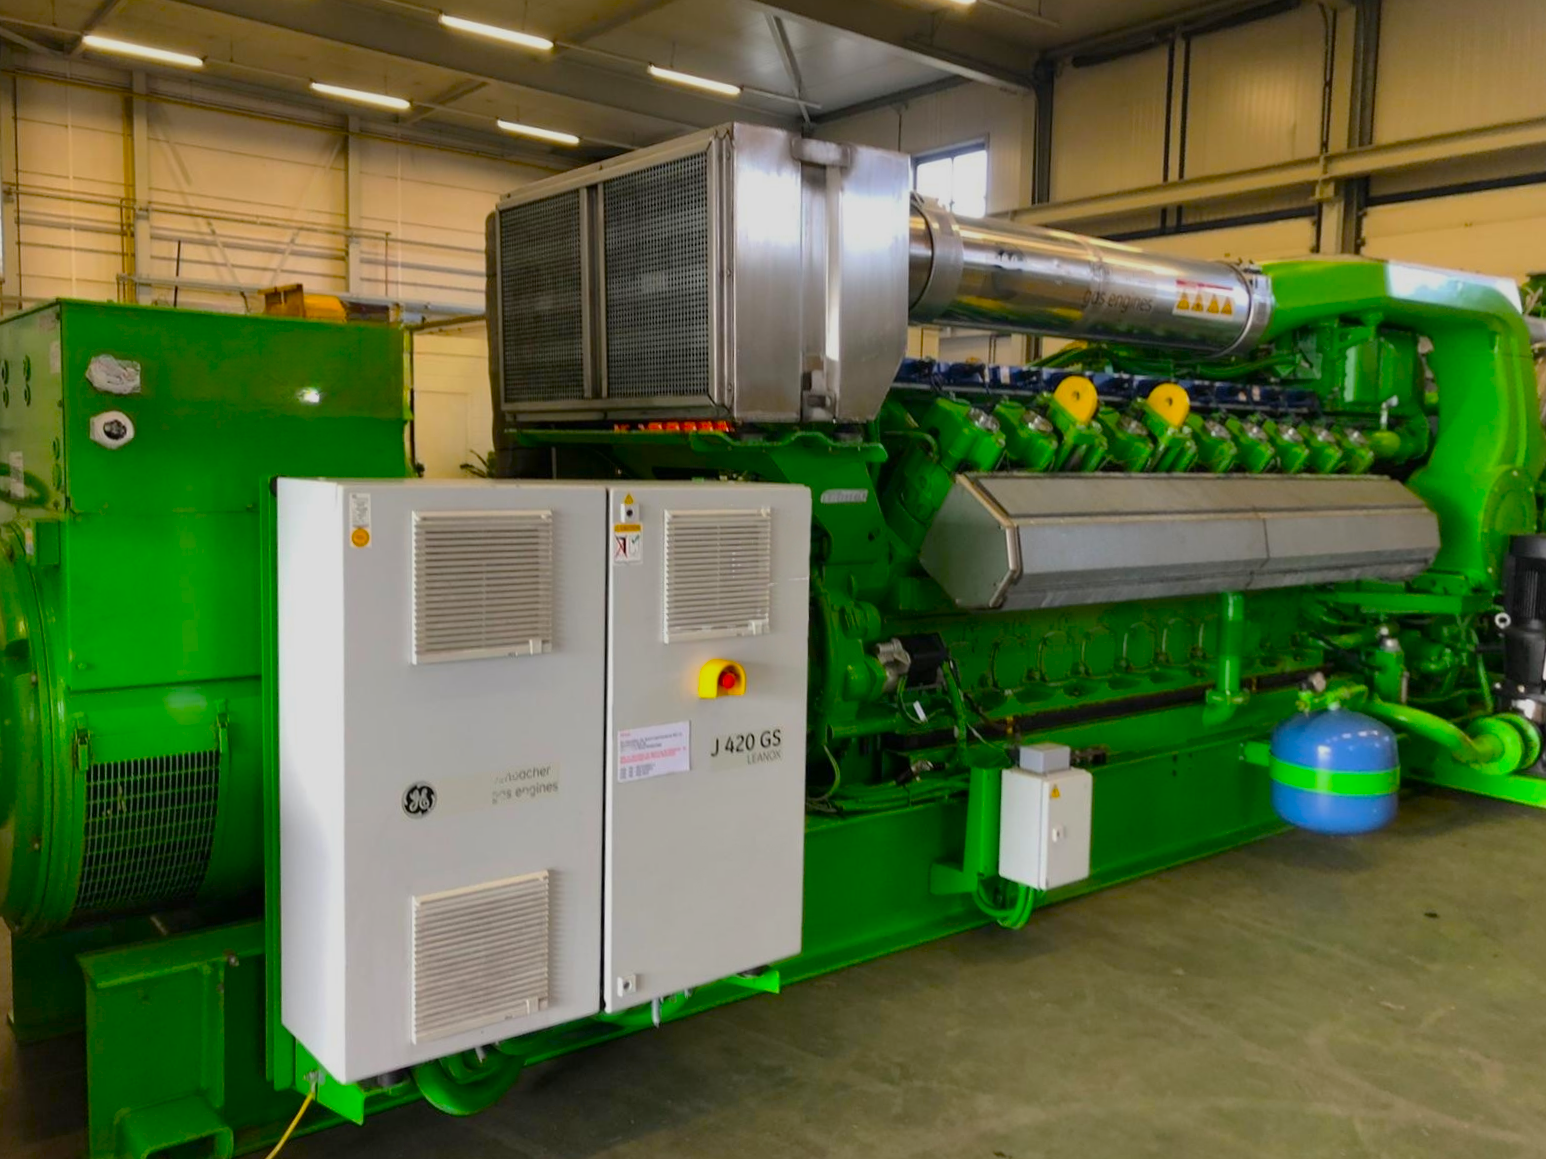
\includegraphics[width=1\linewidth]{figs/gas_gen_j420_leandx.png}
    \caption{Gas powered generator J420 LEANDX}
    \label{fig:gas_gen}
\end{figure}

The gas-powered generator J420 LEANDX, depicted in Figure \ref{fig:gas_gen}, is designed for larger textile manufacturing plants, such as one at which the industrial visit took place. It has a higher capacity and can support extensive machinery and equipment. This type of generator is essential for large-scale operations where the demand for power is significantly higher, ensuring that all processes run smoothly without any interruptions.

Electrical Output
1,411 - 1,562 kW

Thermal Output
1,422 - 1,906 kW

Voltage
480V - 13.8kV

Electrical Efficiency
up to 44.0 %

Thermal Efficiency
up to 50.5 %